\section{Metodology and Results}



\subsection*{3.1 Pump Integration}

    The pump integration in the automation algorithm bring us a new controllable variable, the Flowrate. Now we can control the spraying mode with the
    two main variables that afect the system. 
    It will bring more complexity for the system since now we are dealing with multivariable control.
    Fortunatelly those two variables are uncuppled (* be certain of that first *) which means that actuating in one of them will not interfere in the other one.
    Controlling also the flowrate gives to this project a new dimension in the system giving us freedom to explore the flowrate properties.

    The pump integration was developed using also python language. As I could not find a good library for this pump I developed an quick and easy interface for sending the pump
    commands to be integrated with the main automation routine. The communication with the pump was made using the serial interface and the commands list were found in the pump user manual.


\subsection*{3.2 First mapping Experiments}


    \begin{figure}[H]
        \center
        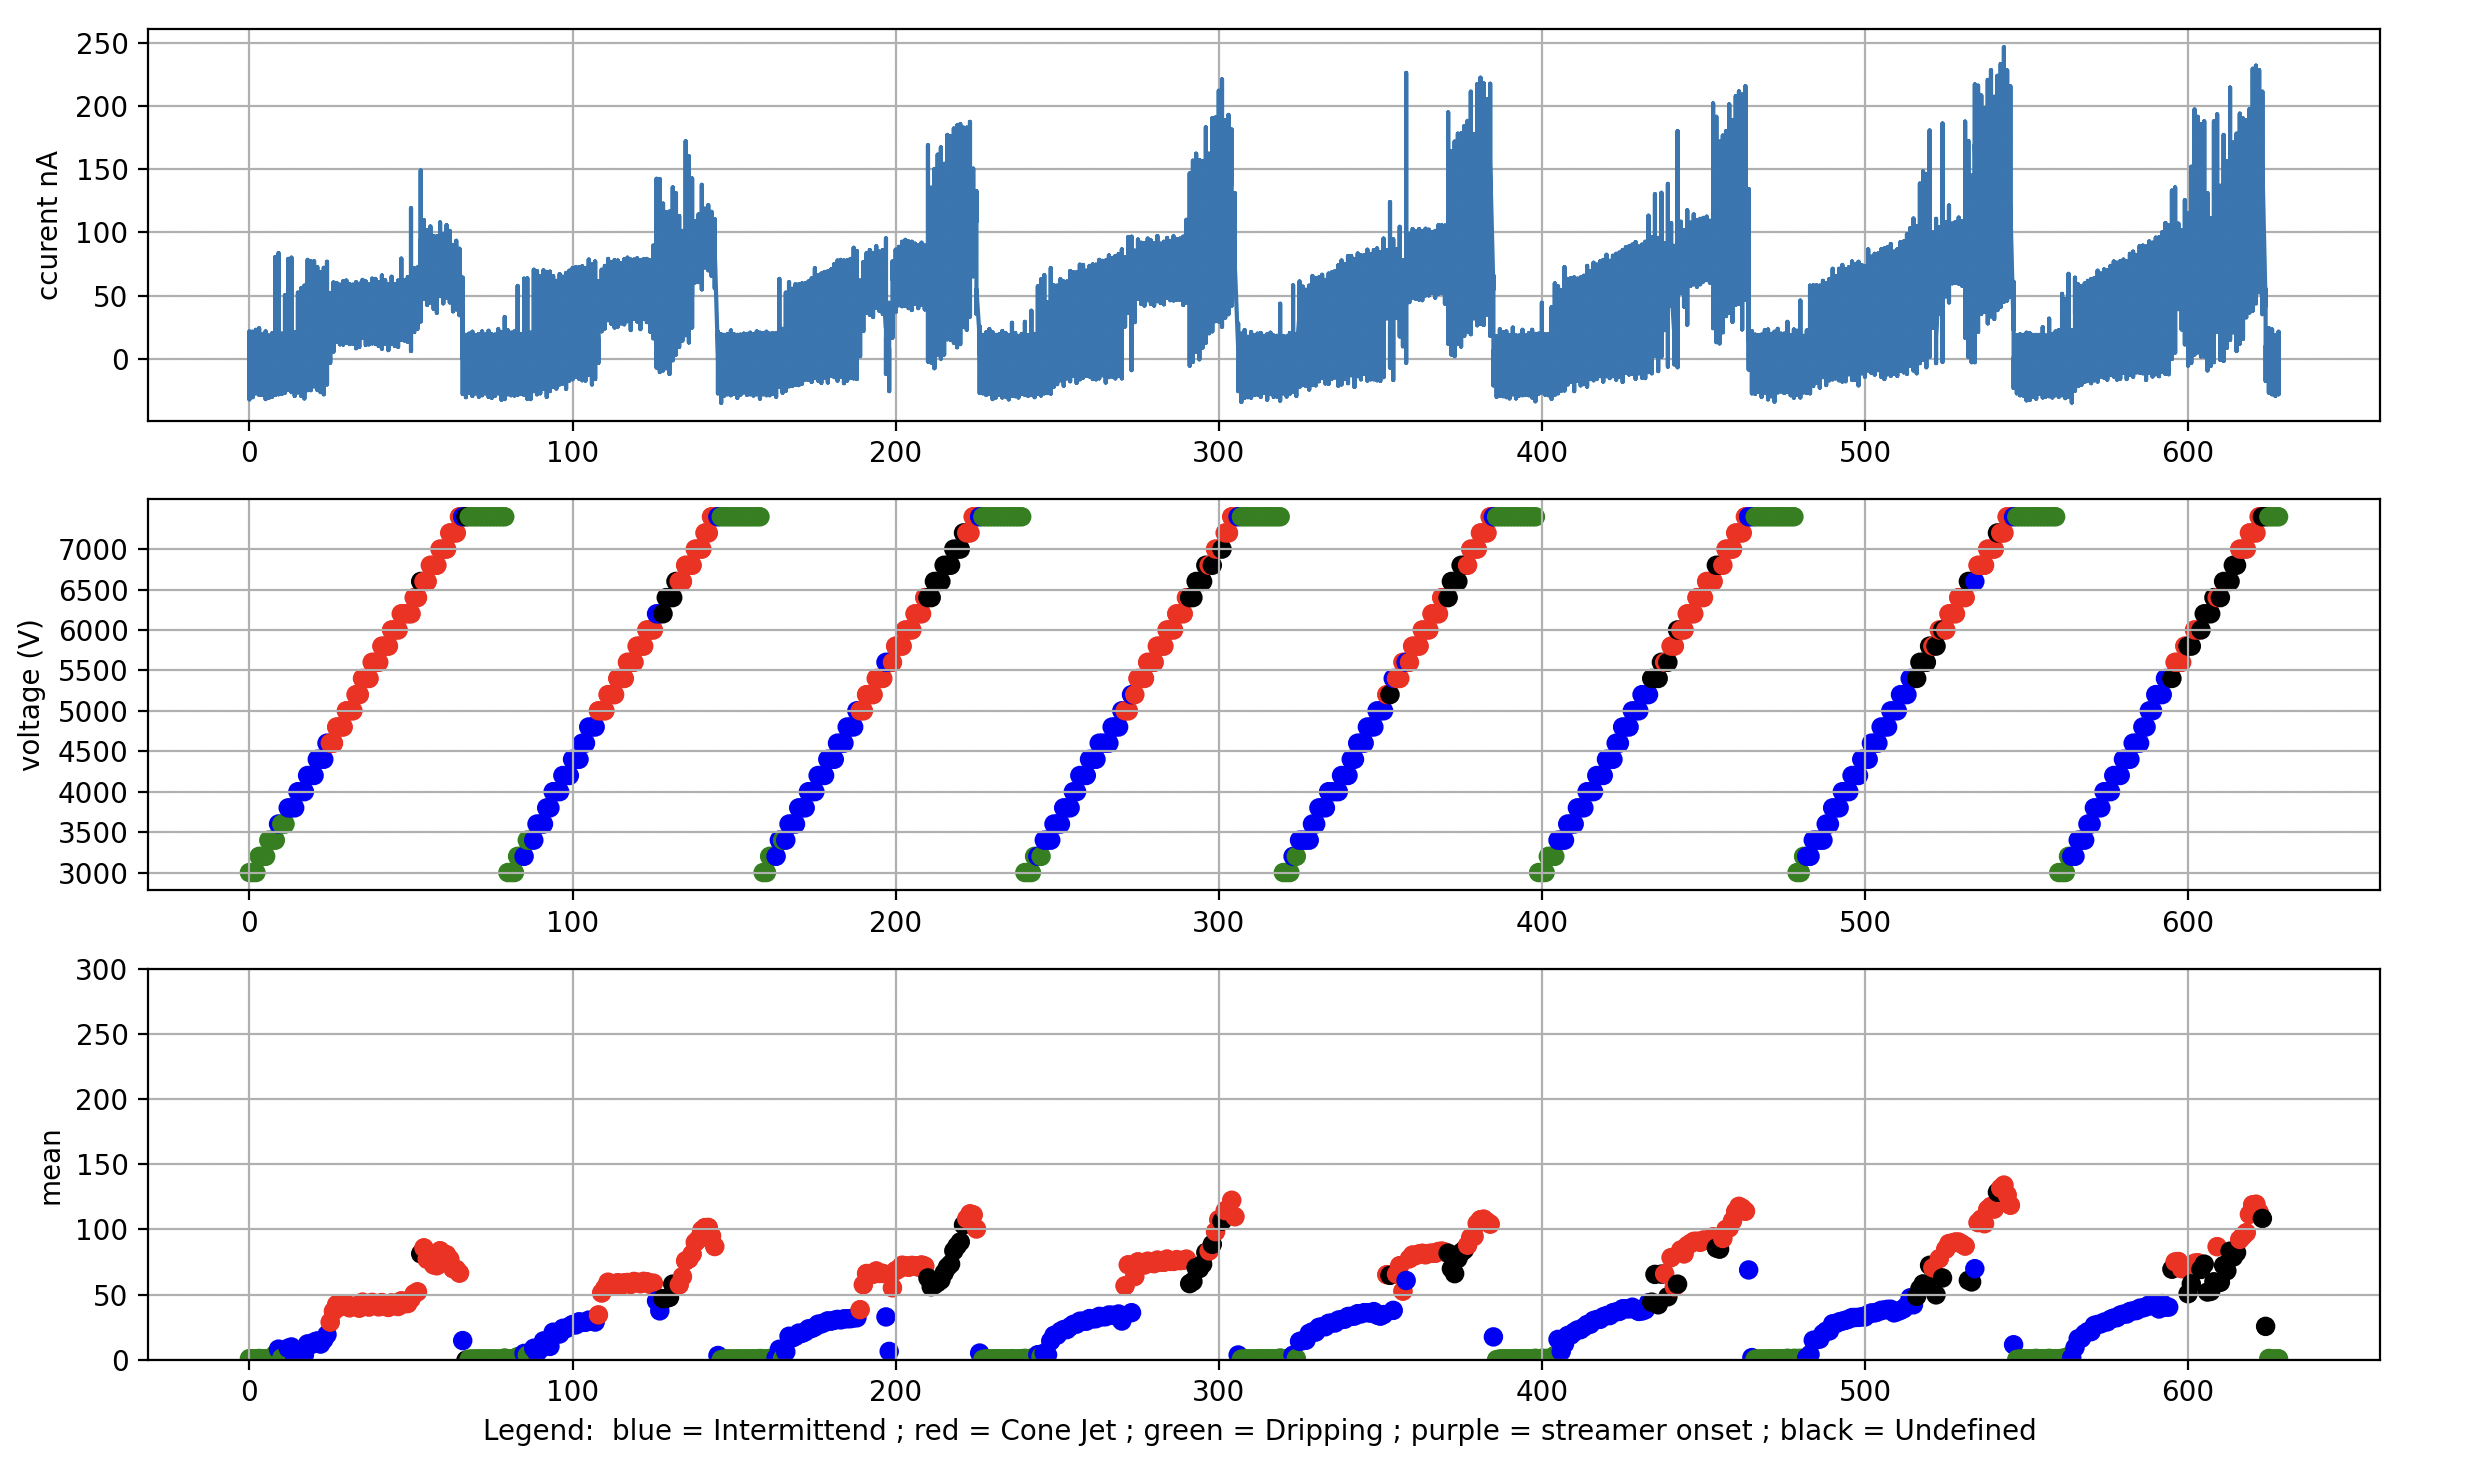
\includegraphics[width=15cm]{images/map2Data.png}
        \caption{Mapping Experiment data}
    \end{figure}

    \begin{figure}[H]
        \center
        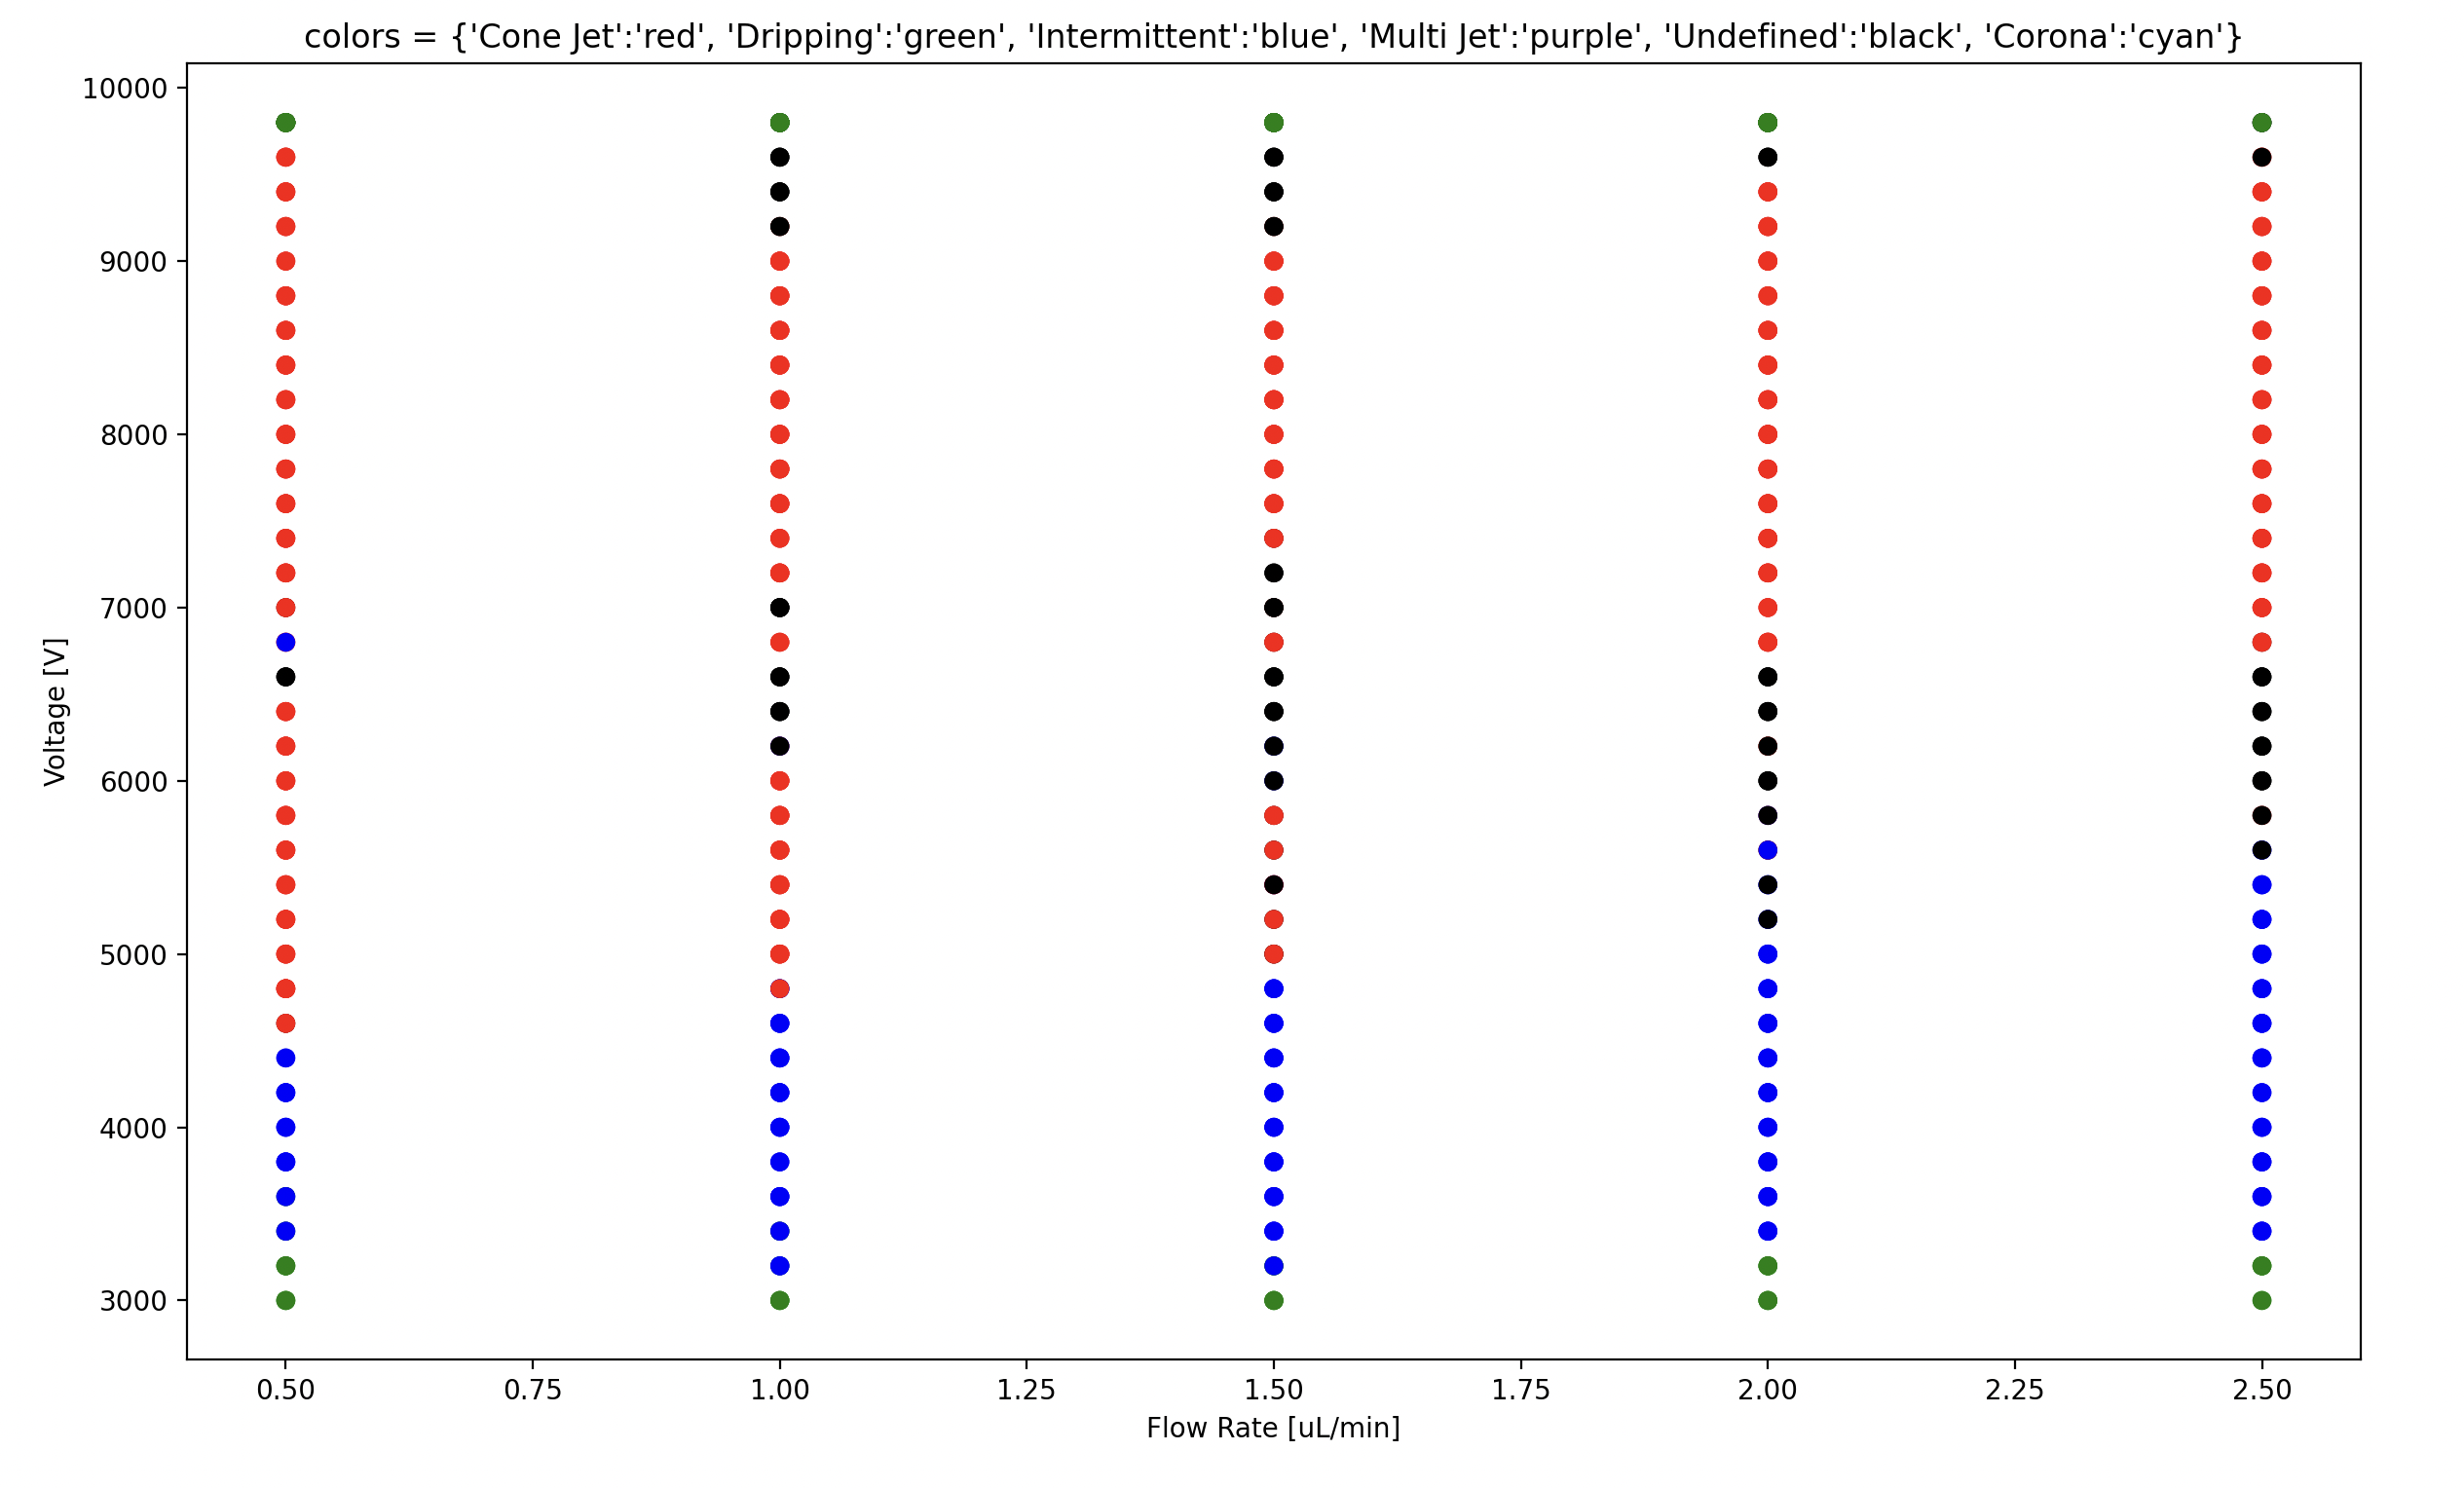
\includegraphics[width=15cm]{images/map1.png}
        \caption{First mapping trial}
    \end{figure}

    \begin{figure}[H]
        \center
        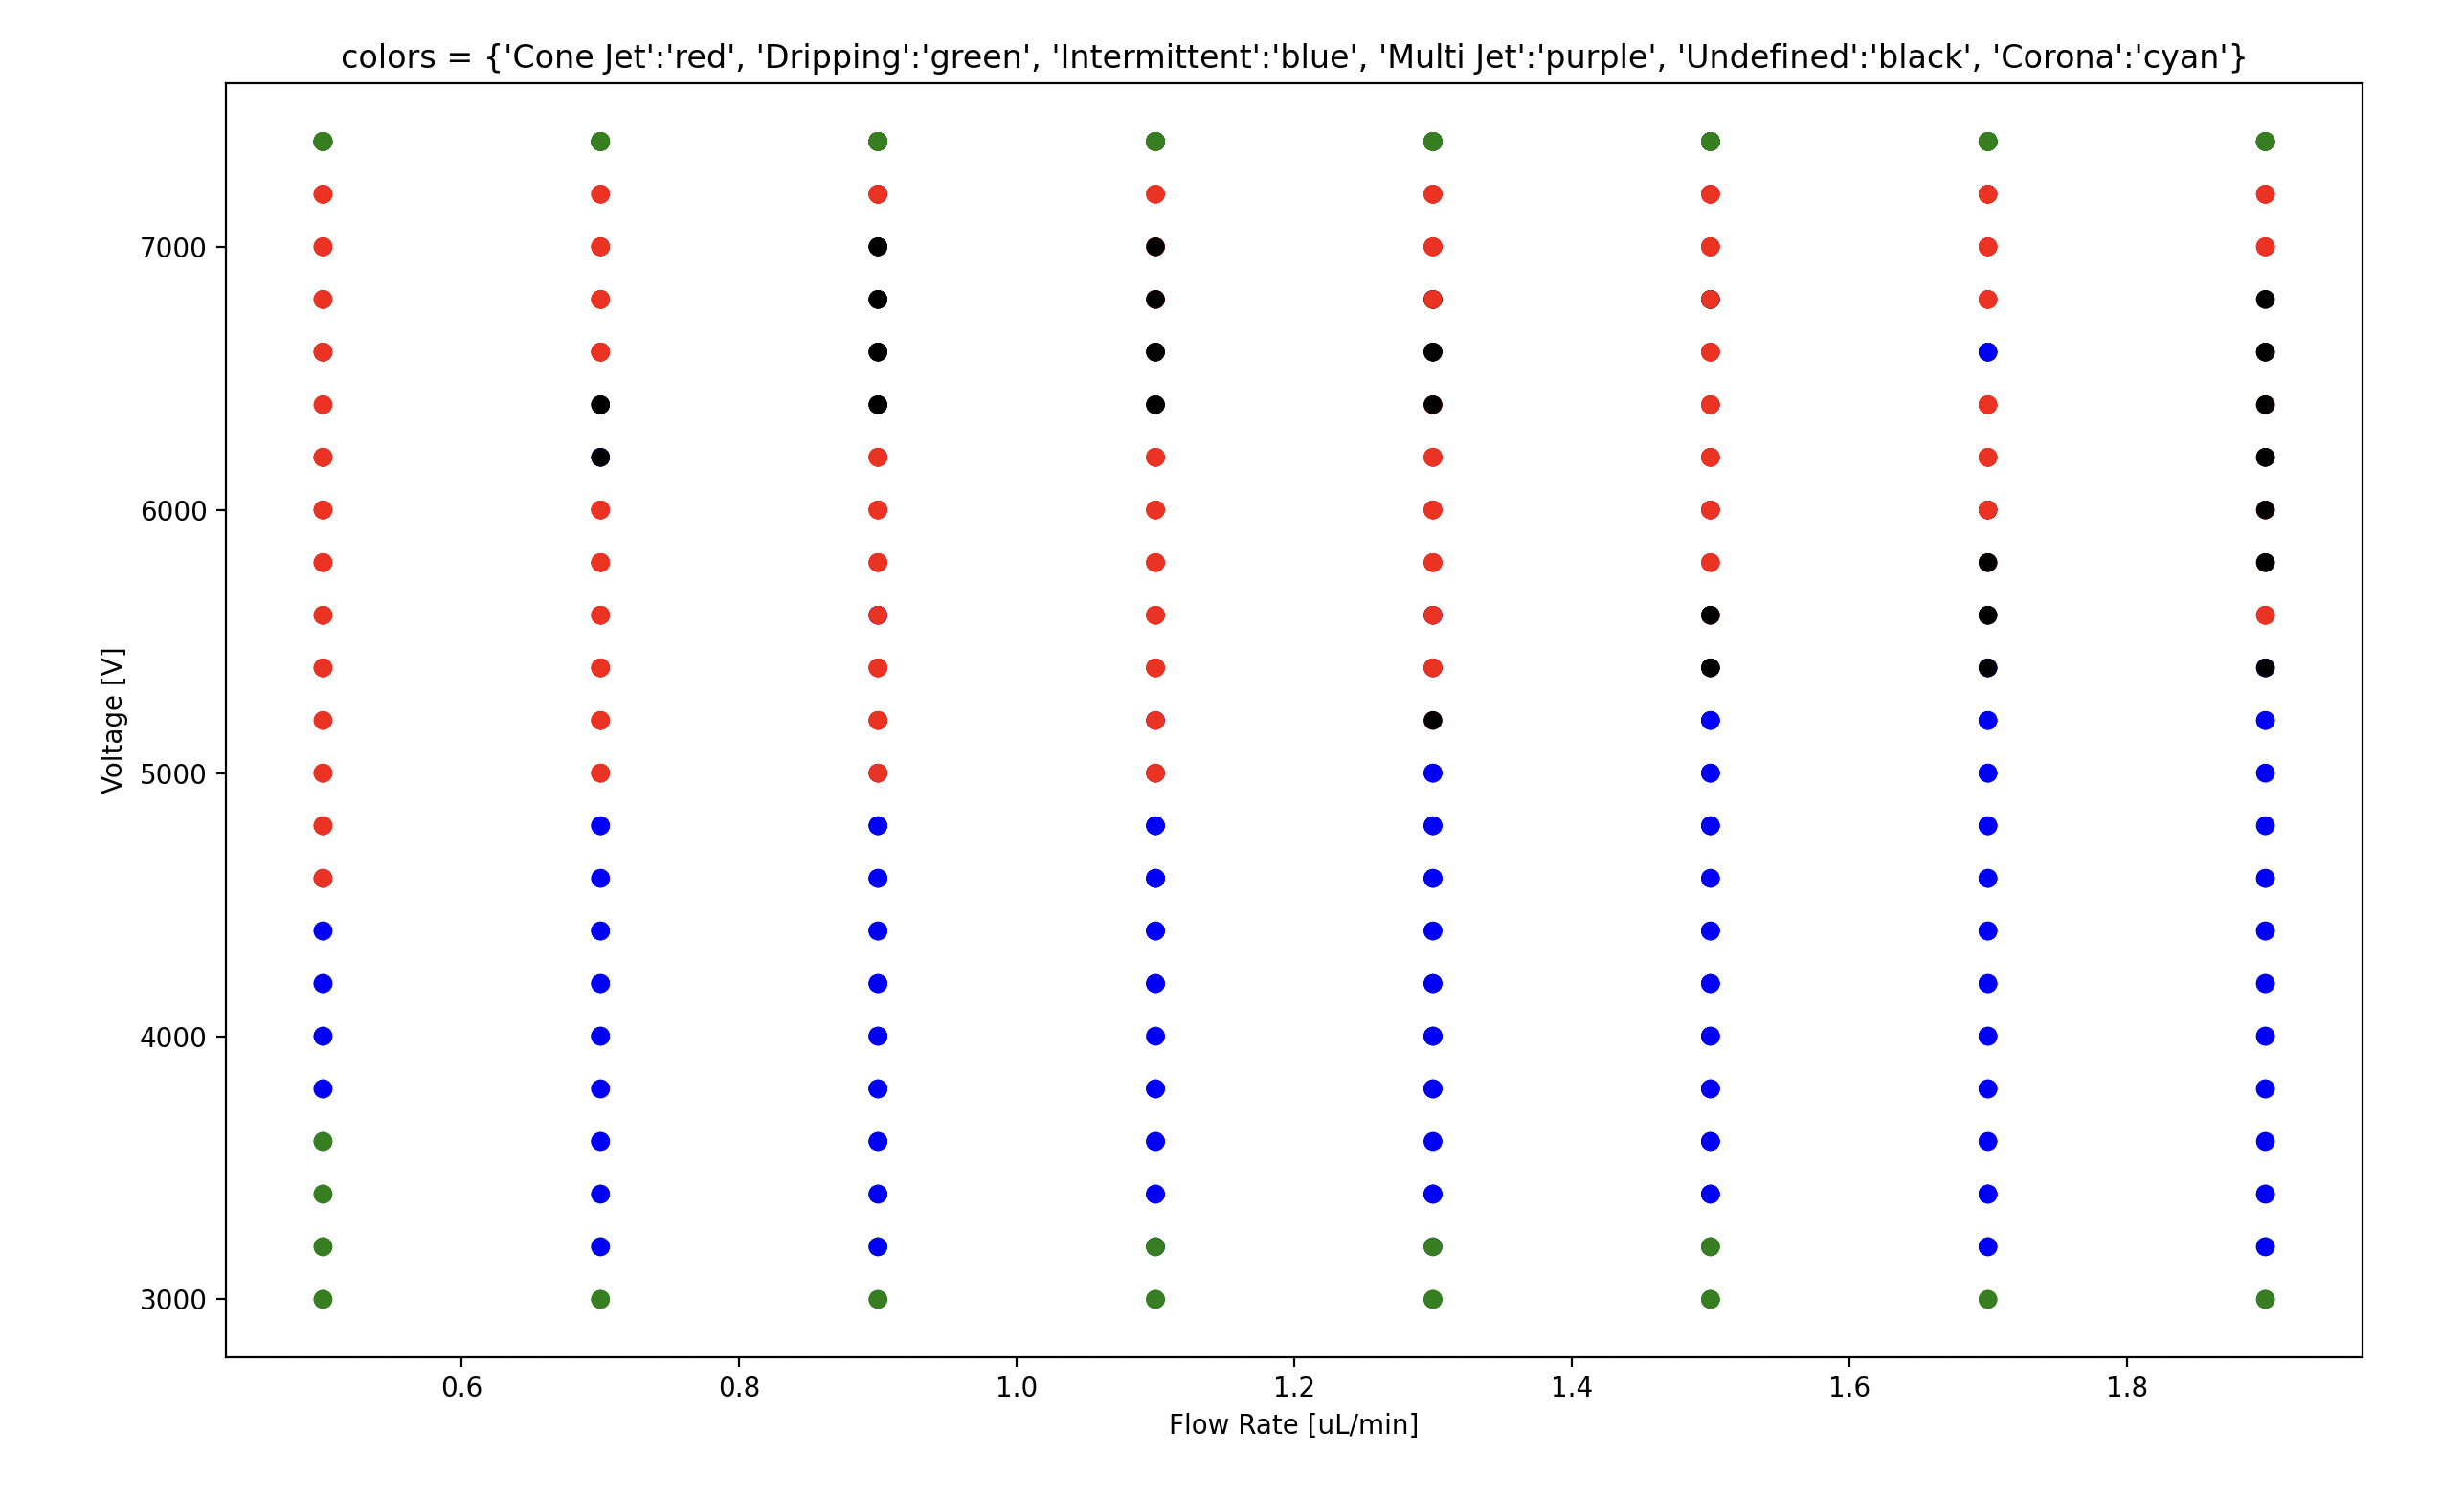
\includegraphics[width=15cm]{images/map2.png}
        \caption{Second mapping trial}
    \end{figure}

    It was noticed that the motor of the pump in certains speed generate a noise caused by the stepping from the stepper motor.
    This noise from the motor was being acquired by the current data and was interfering in the classification method.
    Because of that the firsts results of the map have a lot of undefined or incorrect classifications.
    This can be reduced inserting a bubble in the syringe to atenuate mechanical noises. 


    \begin{figure}[H]
        \center
        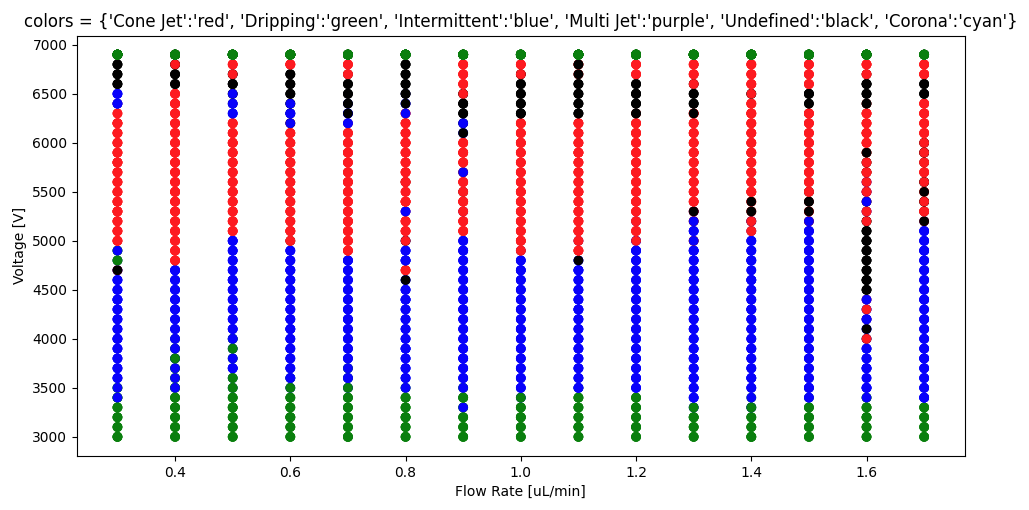
\includegraphics[width=15cm]{images/map3.png}
        \caption{map3}
    \end{figure}






\subsection*{3.3 Step Interference in each sample}


    \begin{multicols}{2}

        \begin{figure}[H]
            \center
            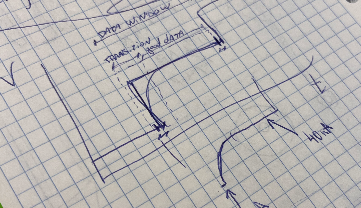
\includegraphics[width=8cm]{images/idea.png}
            \caption{ map3 reproccessed data head }
        \end{figure}



    we were evaluating the interference of each step in the....


        \begin{figure}[H]
            \center
            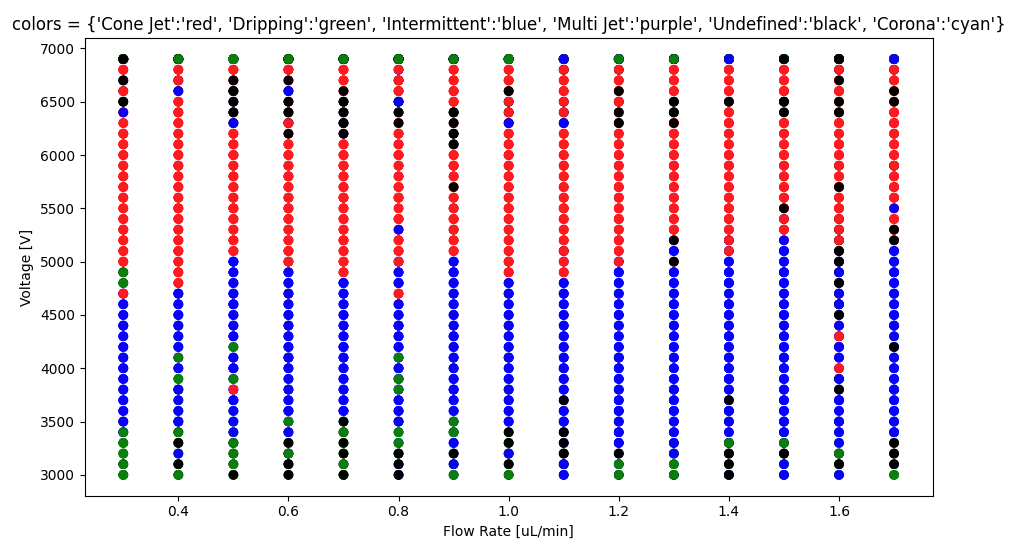
\includegraphics[width=8cm]{images/map3_reproccessed_data_head.png}
            \caption{ map3 reproccessed data head }
        \end{figure}

        \begin{figure}[H]
            \center
            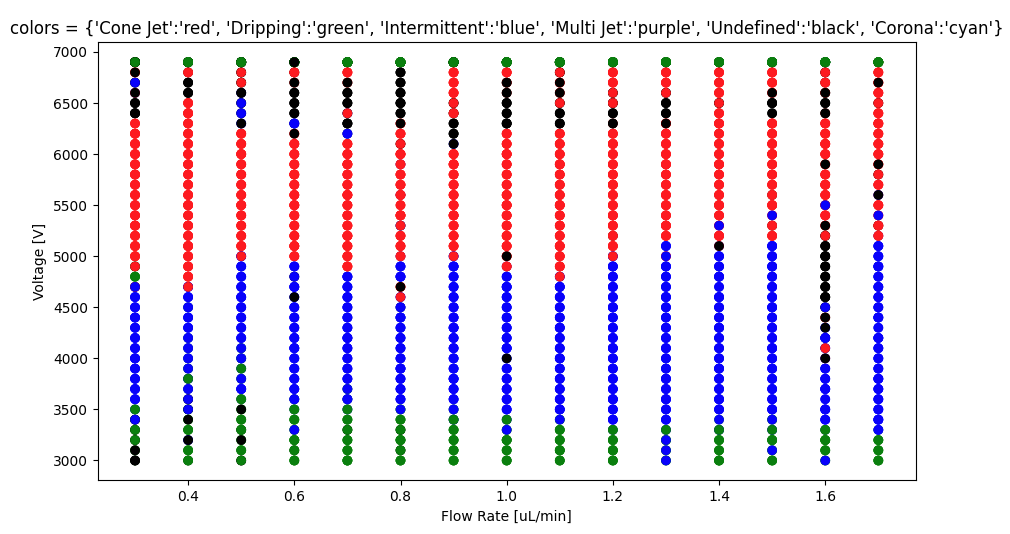
\includegraphics[width=8cm]{images/map3_reproccessed_data_tail.png}
            \caption{ map reproccessed data tail }
        \end{figure}


        \begin{figure}[H]
            \center
            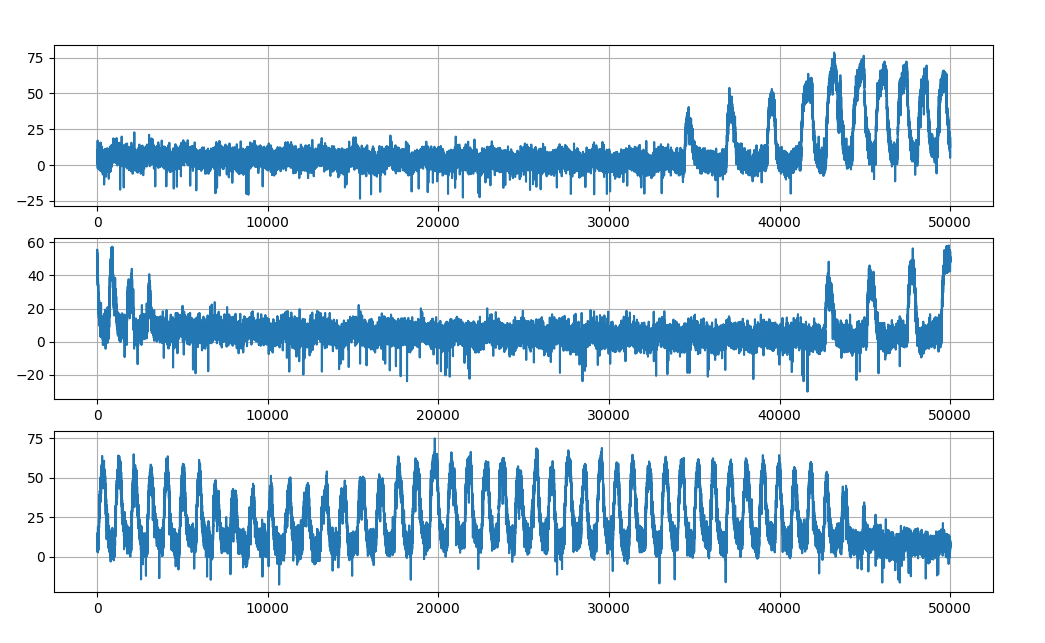
\includegraphics[width=8cm]{images/data_samples.png}
            \caption{ map reproccessed data tail }
        \end{figure}

    \end{multicols}



% \subsection*{3.4 Experiment 3}

%     - liquid: ethanol pure
        
%     - flow rate min: 1.5 mL/hr

%     - camera to nozzle distance: 16.5 cm

%     - config: nozzle to plate

%     - nozzle to plate or ring distance: 1.5 cm

%     - nozzle diameter: 0.136 mm

%     - type of measurement: 

%         * voltage start: 3000 V

%         * voltage stop: 11000 V

%         * step size: 50 V 

%         * step time: 1 s

